\documentclass[10pt]{beamer}

\usepackage{graphicx}

\usetheme{metropolis}
\usepackage{appendixnumberbeamer}

\usepackage{booktabs}
\usepackage[scale=2]{ccicons}

\usepackage{pgfplots}
\usepgfplotslibrary{dateplot}

\usepackage{xspace}
\newcommand{\themename}{\textbf{\textsc{metropolis}}\xspace}

\title{A Future Persepective:}
\subtitle{Exploiting Decentralized Web for Pragmatic Interoperability}
\date{November 21, 2018}
\author{\textbf{Dr. Bambang Purnomosidi}}
\institute{Informatics Engineering Department\\STMIK AKAKOM}
\titlegraphic{\hfill
\includegraphics[height=1.5cm]{isriti-logo.png}}

\begin{document}

\maketitle

\begin{frame}[allowframebreaks]{Table of contents}
  \setbeamertemplate{section in toc}[sections numbered]
  \setbeamertemplate{subsection in toc}{\leavevmode\leftskip=3.2em\rlap{\hskip-2em\inserttocsectionnumber.\inserttocsubsectionnumber}\inserttocsubsection\par}
  \tableofcontents
  %\tableofcontents[hideallsubsections]
\end{frame}

\section{Introduction}

  \subsection{Overview}

    \begin{frame}[fragile]{Overview}

  The World Wide Web (or the Web) is currently consists of many technologies, ecosystems, and virtual resources. Until now, most interactions on the Web happen between client and server. This situation leads to centralized Web where organzations and / or people put their services on the Web for mass consumption by clients. While this situation is normal, centralized Web gives negative impacts for society. Centralized Web gives power to service provider. By building Web to a more decentralized system, we may put power into clients / peers, therefore opening possibilities for customization and interoperability. The decentralized Web empowers creation and encourages participation, hence enable people to create, personalize, and share resources. This talk is a glimpse into pragmatic interoperability by exploiting possibilities from decentralized Web and how we might put pragmatic interoperability into our resources on the (decentralized) Web for the benefit of society as a whole.

    \end{frame}

  \subsection{Web and Decentralized Web}

    %\begin{frame}[allowframebreaks]{Web and Decentralized Web}
    \begin{frame}[allowframebreaks]{Web and Decentralized Web}

      \begin{itemize}
        \item Web is a platform which consists of front end resources (HTML, CSS, pictures, videos, JavaScript), rendered by Web browser. Those resources might be static or produced by backend processing. 
        \item Current Web is distributed but mostly have centralized points of control.
        \item This situation puts people in weak position compared with government, private companies or any other big organization. Sensor and surveillance from government are possible. Private companies may use people's data without their consent.
        \item Many layers for people who want to create services and participate.
      \end{itemize}


    \end{frame}

  \subsection{Interoperability}

    \begin{frame}[fragile]{Interoperability}

      asdsdfsdf

    \end{frame}

\section{Interoperability on the Web}

  \subsection{Syntactic Interoperability on the Web}

    \begin{frame}[fragile]{Syntactic Interoperability on the Web}
      sf
    \end{frame}

  \subsection{Semantic Interoperability on the Web}

    \begin{frame}[fragile]{Semantic Interoperability on the Web}
      Semantic interoperability is achieved when both side can exchange semantic data. 
    \end{frame}

  \subsection{Interoperability and Decentralized Web}

    \begin{frame}[fragile]{Interoperability and Decentralized Web}
      sf
    \end{frame}

\section{Pragmatic Interoperability and Decentralized Web}

  \subsection{Requirements for Pragmatic Interoperability}

    \begin{frame}[fragile]{Requirements for Pragmatic Interoperability}

      \begin{itemize}
        \item Pragmatics: study how context contributes to meaning. The ability to understand pragmatic in conversation is called \textbf{pragmatic competence}.
        \item Client and service provider is said to be capable of doing contextual and pragmatic interactions if both side can accommodate context in conversation and both understand intention of each side within the same context.
      \end{itemize}

    \end{frame}

  \subsection{Architecture of Decentralized Web Components for Pragmatic Interoperability}

    \begin{frame}[fragile]{Architecture of Decentralized Web Components for Pragmatic Interoperability}

      \begin{figure}[h]
      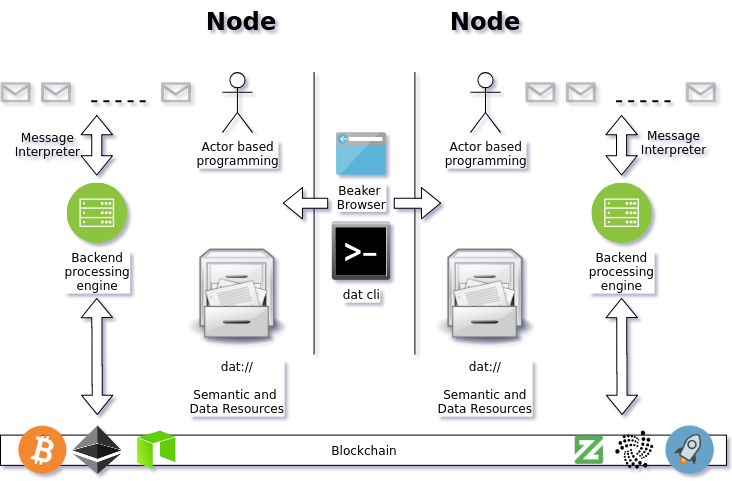
\includegraphics[scale=0.4]{decweb-pragmatic-int}
      \end{figure}

    \end{frame}

  \subsection{Impact for Society}

    \begin{frame}[fragile]{Impact for Society}
      \begin{itemize}
        \item More powerful clients, providing balance of power between any entities and people.
        \item Difficult for censorship and surveillance
        \item Robust: there is no single node which can take the whole network down.
        \item Eliminate middleman, hence reduce costs and complexities
        \item There are possiblities 
      \end{itemize}
    \end{frame}

  \subsection{Research Challenges}

    \begin{frame}[fragile]{Research Challenges}
      \begin{itemize}
        \item Identity
        \item Context taxonomy
        \item Actor-based programming tools
        \item Message interpreter
        \item Semantic infrastructure
        \item Interledger protocol
      \end{itemize}
    \end{frame}

\end{document}
